\subsection{Prototype}

From the list of features mentioned in the previous chapter we have selected the most important ones and created a prototype in a form of MVP (Minimum Viable Product). 

The selected features:

\begin{enumerate}
	\requirement{3}{load an Instruction}
	\requirement{3}{view the 3D representation of the Instruction step}
	\requirement{3}{switch to the next step in the Instruction}
	\requirement{3}{switch to the previous step in the Instruction}
	\requirement{3}{see the Transition between two Instruction steps}
	\requirement{2}{pause the Transition at any time}
	\requirement{2}{rewind the Transition}
	\requirement{2}{forward the Transition}
	\requirement{3}{rotate the Model in 3D space}
	\requirement{3}{zoom the Model in and out in 3D space}
	\requirement{1}{see creases of the Model} 
	\requirement{2}{distinguish paper's top and bottom sides} 
\end{enumerate}

Some of the listed functionalities require a numerical solver which is also included in the MVP.

Both Instructions and Transitions are represented using .fold files which we have extended with information required by the application.

\subsubsection{Frontend}

At first we had decided to use plain \tech{JavaScript} with the \tech{Rollup} bundler and \tech{Three.js} framework.
It quickly became apparent that the lack of state management will become problematic as the development progresses. Following that realization we have decided to incorporate a reactive framework - \tech{React} to aid the project with basic layout and aforementioned state manipulation. 
Due to minor interoperability issues the Rollup was also replaced with \tech{Webpack}.

The quality assurance is achieved through the use of:

\begin{description}
\item[Code linter] - EsLint
\item[Code prettiefier] - Prettier
\item[Test Runner] - Jest
\item[Continuous integration] - Github Actions
\end{description}

The implementation is continuously delivered to \tech{Netlify} via Github Actions.


\begin{figure}[H]
\caption{Origami simulation view}
  \centering
    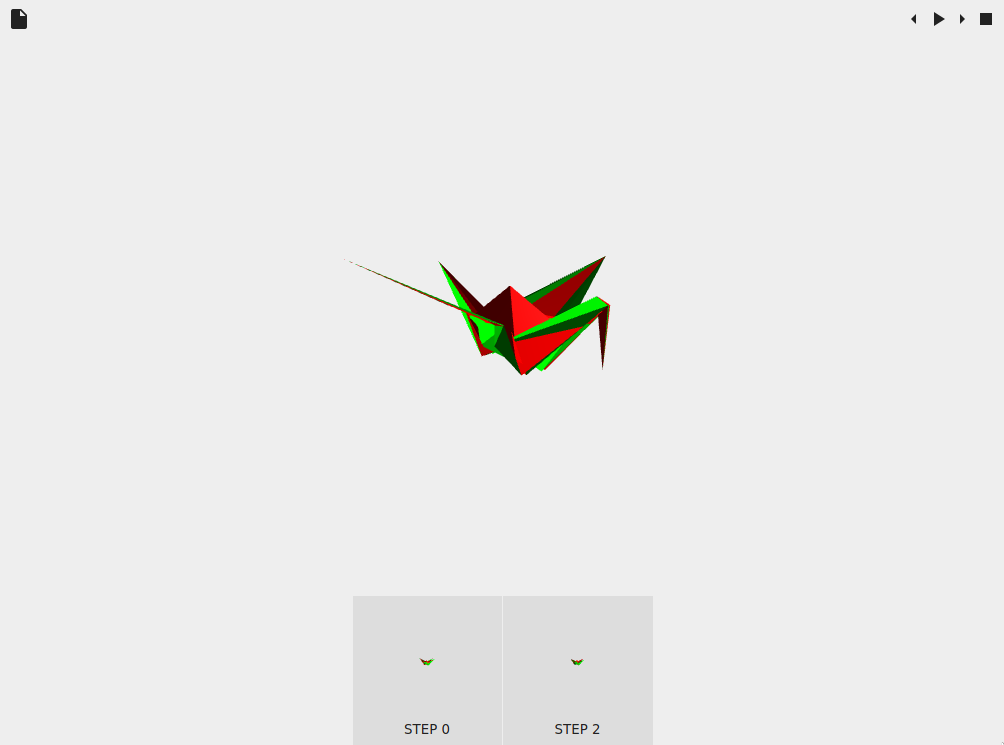
\includegraphics[width=0.8\textwidth]{assets/prototype-front.png}
\end{figure}

\subsubsection{Backend}

The current backend part is responsible for carrying out numerical computations.
It converts a provided Instruction into a set of coordinates representing
transitions between folding steps.\\

The solver is based on the techniques presented in the publication by A. Ghassaei.\cite{origami-simulator}.

The computational framework consists of the three most important forces,
that drive the folding process.

\begin{description}
	\item[Beam force] - responsible for preserving edge length
	\item[Face force] - responsible for preserving the original face shape
	\item[Crease force] - responsible for folding
\end{description}

Given the current vertices' positions, and the mountain-valley assignment,
the solver computes forces imposed on vertices, and calculates their next position
using the forward Euler integration.

An additional \textbf{damping force} is introduced to prevent solver from
high frequency oscilations, assuring numerical stability under most conditions.\\

The solver is implemented in \tech{python}, using \tech{numpy} and \tech{scipy} libraries. 


\begin{figure}[H]
	\caption{Visualization of vertices (dots), and forces applied to them (arrows)
	during folding of a rectangular sheet of paper in half, along the diagonal. }
  \centering
    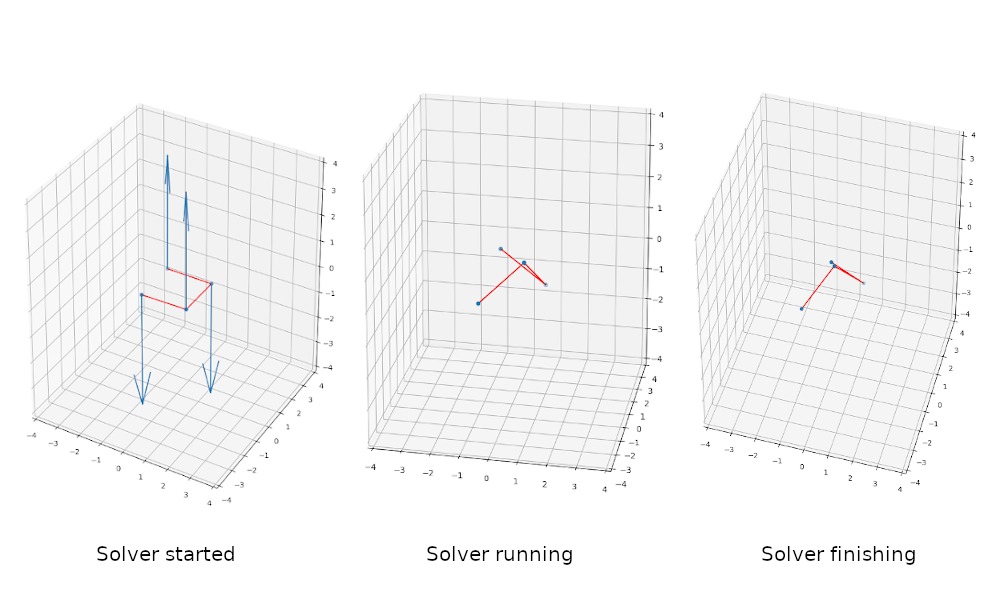
\includegraphics[width=0.8\textwidth]{assets/prototype-backend.png}
\end{figure}


\subsection{Project overview}

\begin{figure}[H]
	\caption{High level system overview}
  \centering
    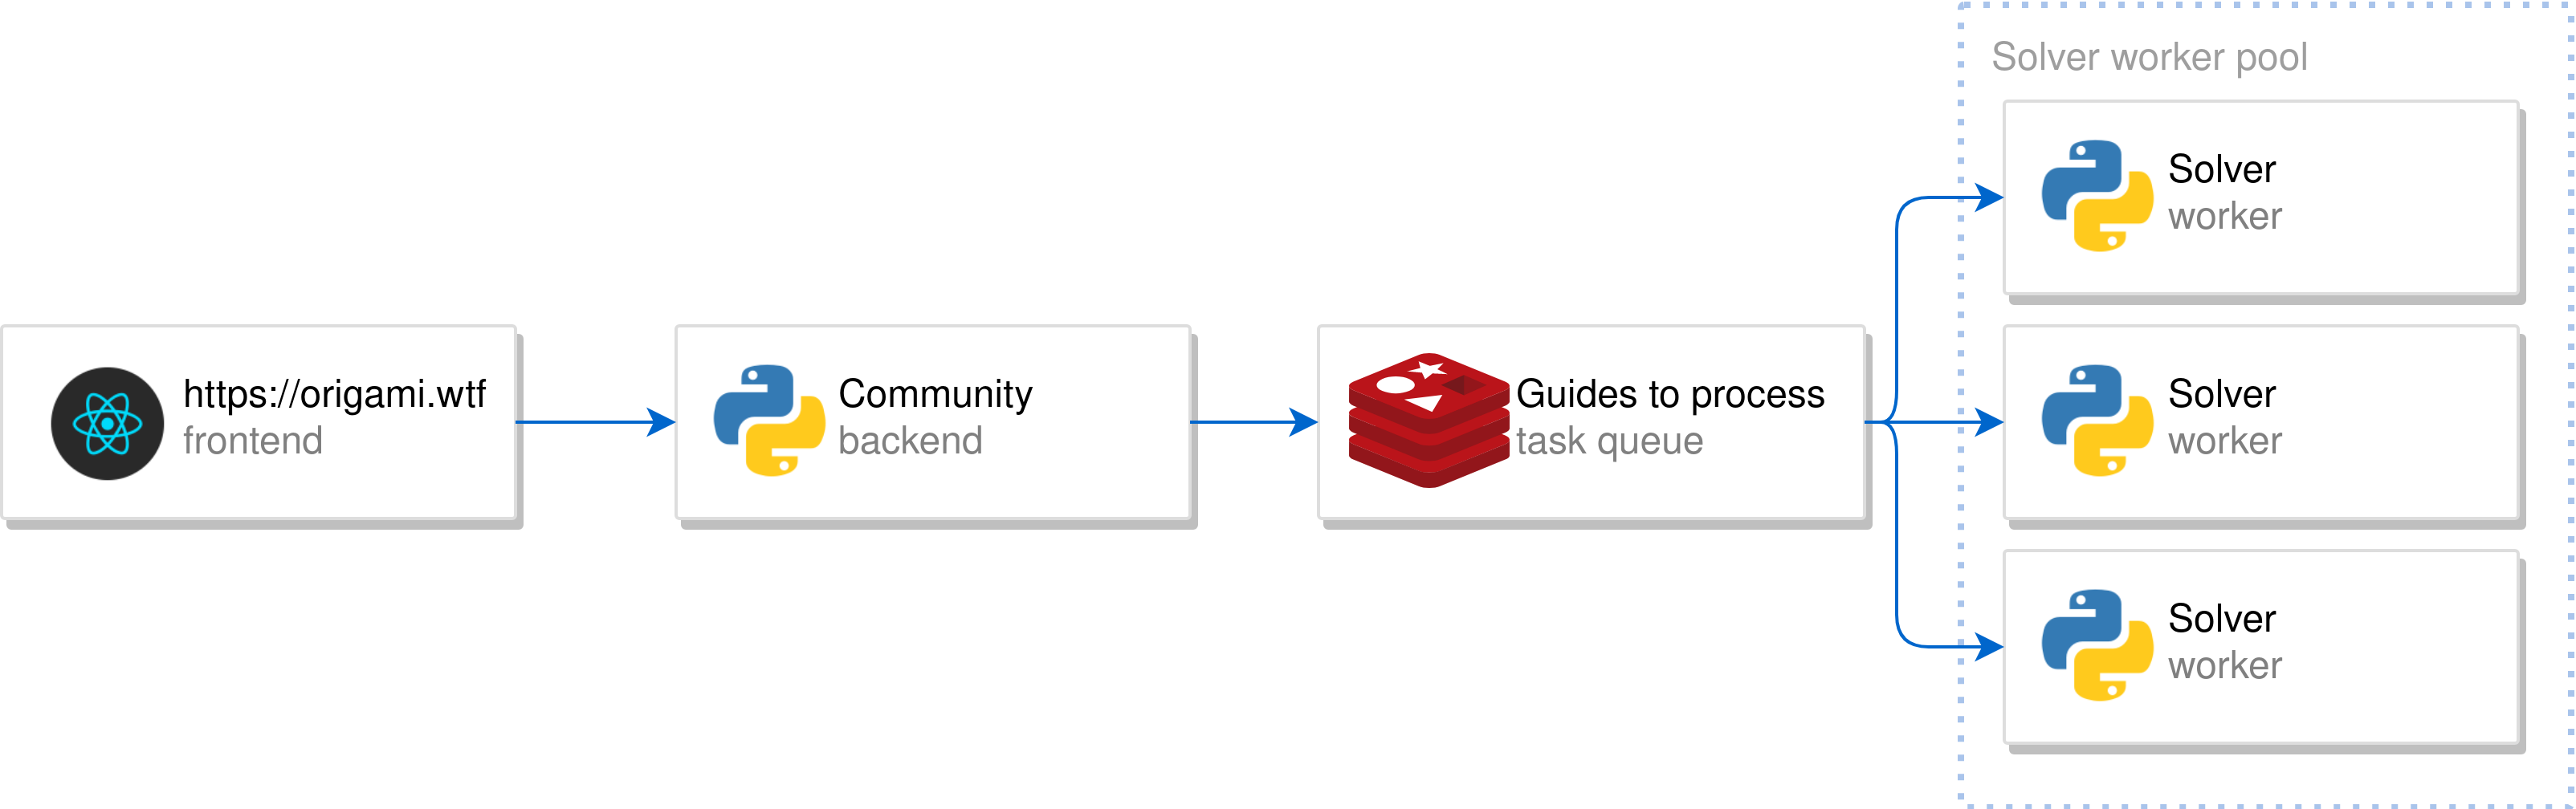
\includegraphics[width=\textwidth]{assets/architecture.png}
\end{figure}

Origuide consists of the following layers:
\begin{description}
	\item[Frontend] - a component that handles all user interactions with the system. 
	\item[Backend] - a component responsible for: \begin{itemize}
		\item processing all user requests initiated on the Frontend
		\item managing persistent data 
		\item authentication and authorization
		\item scheduling Guide processing
	\end{itemize}
	\item[Guides to process] - a task queue distributing guides to process among Solver workers
	\item[Solver worker] - a component responsible for converting Instructions to Guides.
\end{description}

As we previously distinguished two types of users in the system, there are two main success paths through the application.

\begin{figure}[H]
	\caption{Designer's success path}
  \centering
    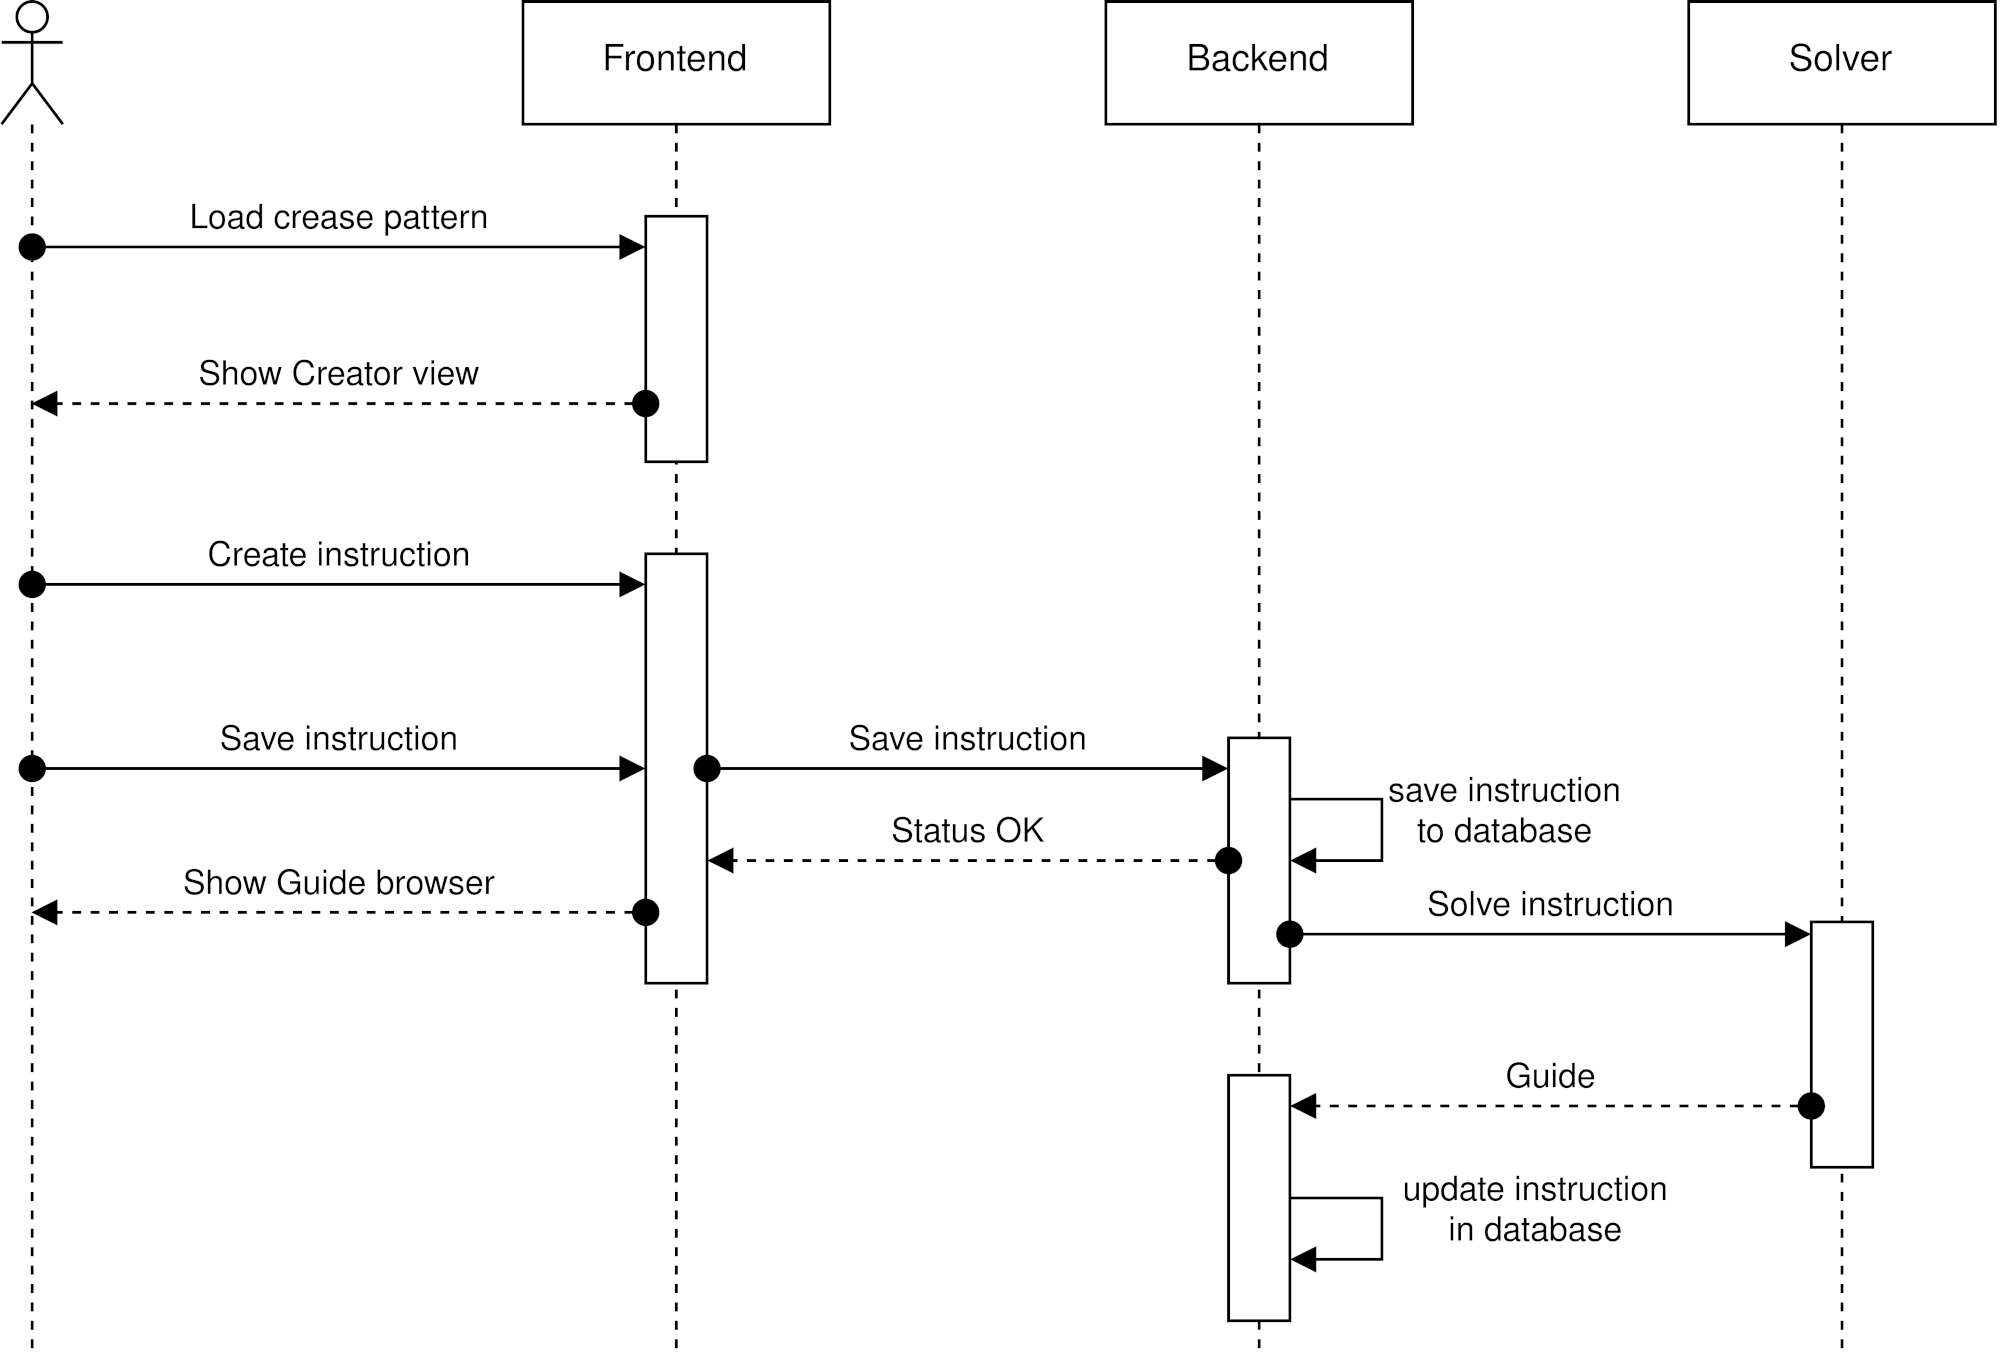
\includegraphics[width=\textwidth]{assets/3-designer-flow.png}
\end{figure}

Designer's main objective is to create Guides. After uploading a Crease Pattern, Designer is required to provide instruction steps. When an Instruction is saved it gets scheduled on a Task Queue and processed by a Solver worker. Once processing is finished the Instruction associatied with the Guide is marked as solved in the database.

\begin{figure}[H]
	\caption{Folder's success path}
  \centering
    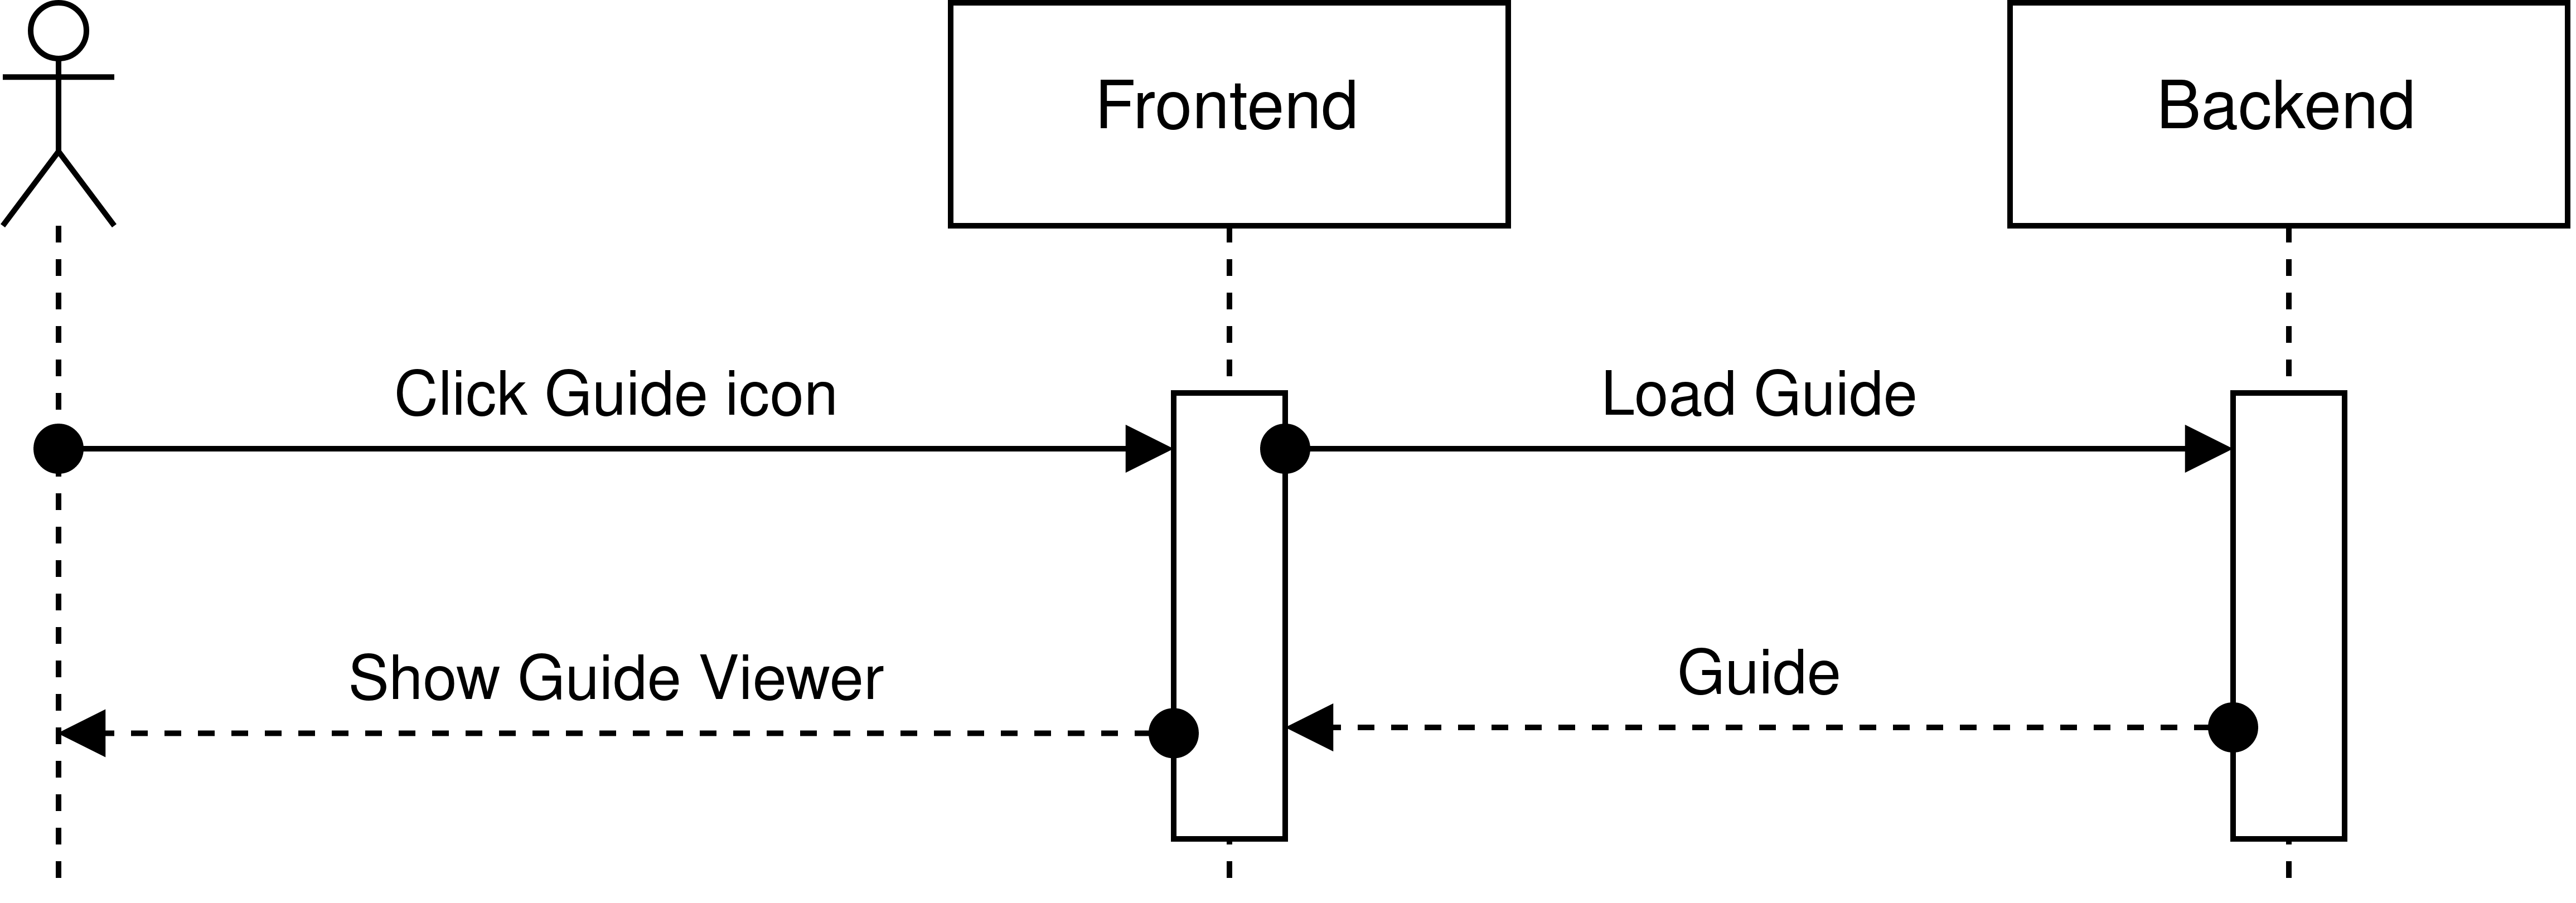
\includegraphics[width=\textwidth]{assets/3-folder-flow.png}
\end{figure}

Folder's main objective is to fold origami figures following steps presented by the Application. After successfully retrieving a guide from the Backend, he is presented with a Guide Viewer.

\subsection{Technology stack}

Source Code is version controlled using a hosted \tech{Git} solution - \tech{Github}.  

Continuous Integration and Continuous Deployment is provided by \tech{Github Actions}. 

\subsubsection{Frontend}

\begin{itemize}
	\item The Application is built in \tech{Javascript} using \tech{React} framework. 
	\item \tech{Three.JS} is used to display 3D models.
	\item Triangulation is done using \tech{earcut}. 
	\item Parsing folds is aided by \tech{fold}.
	\item User Interface components come mainly from \tech{material-ui}.
	\item \tech{Webpack} is responsible for bundling, minimizing and transpiling the source code.
	\item Code style is checked using \tech{Prettier} with \tech{eslint} and enforced on every commit using \tech{Husky}.
	\item \tech{Jest} has been incorporated as a test runner.
\end{itemize}

// TODO: comment

\subsubsection{Backend}

\begin{itemize}
	\item The Backend is built in \tech{Python} using \tech{Django} framework. 
	\item \tech{DjangoRestFramework} simplifies a REST server setup.
	\item \tech{drf-base64} helps with decoding of base64 encoded files.
	\item \tech{PyJWT} assists in auth process.
	\item \tech{factory-boy} is used to generate testing data.
	\item Data is stored in a \tech{PostgreSQL} database.
	\item \tech{Celery} was chosen for an asynchronous task processing.
	\item \tech{Redis} acts as a task queue for \tech{Celery}.
\end{itemize}


\subsubsection{Solver}

\begin{itemize}
	\item Solver runs under \tech{Python}'s alternative implementation - \tech{PyPy}.
	\item \tech{Shapely} is used for triangulation.
\end{itemize}



\subsection{Components overview}
% Przegląd poszczególnych komponentów a wiec np. baza danych, aplikacja typu klient, serwis RESTowy. Jeśli baza to ERD z opisem, jeśli aplikacja kliencka to jakie elementy, widoki, jak się łączy i kiedy. Jeśli prosta aplikacja WWW to można pokazać strukturę projektu. Jeśli serwis RESTowy to jego specyfikacja z przykładami. Protokół komunikacji to może być zupełnie osobny opis. %

\subsection{Algorithms}
% Ciekawsze algorytmy, aspekty, mechanizmy np. logowanie, indeksowane, cachowanie, synchronizacja, backup, jakieś procesy w tle, jakieś progress bary, jakieś analizy, generowanie warstw GISowych, lokalizacja etc. Jest tu często o czym pisać. %

\subsection{Development environment setup}
% Instrukcja postawienia środowiska deweloperskiego - jeśli potrzeba wypełniacza %

\subsection{Deployment}
% Instrukcja postawienia środowiska deweloperskiego - jeśli potrzeba wypełniacza %

\subsection{Quality assurance}
% Quality Assurance: czy mamy testy jednostkowe? Czy mamy inne testy automatyczne? Jakich bibliotek używacie? %
At every commit that is a part of the master branch or a Pull Request Unit Tests are run. \\

\subsection{Problems encountered}
% Z jakimi problemami technicznymi sie borykaliście? Jeśli nie opisaliście ich w dokumentacji procesowej. %

